\documentclass[10pt,a4paper]{article}
\usepackage[margin=2cm]{geometry}
\usepackage{mathptmx}
\usepackage{amsmath}
\usepackage{booktabs,longtable,array}
\usepackage{graphicx}
\usepackage{xspace}
\usepackage[hyphens]{url}
\usepackage{hyperref}
\graphicspath{{../figures/}}
% Generated by code/make_manuscript_numbers.py -- do not edit by hand.
\newcommand{\BenchAmbiguous}{13}
\newcommand{\BenchCorrectPmg}{48}
\newcommand{\BenchCorrectVone}{51}
\newcommand{\BenchCorrectVoneFb}{51}
\newcommand{\BenchCorrectVtwo}{50}
\newcommand{\BenchCorrectVtwoGr}{50}
\newcommand{\BenchExactPmg}{38}
\newcommand{\BenchExactVone}{38}
\newcommand{\BenchExactVoneFb}{38}
\newcommand{\BenchExactVtwo}{37}
\newcommand{\BenchExactVtwoGr}{37}
\newcommand{\BenchFalseRefPmg}{0}
\newcommand{\BenchFalseRefVone}{0}
\newcommand{\BenchFalseRefVoneFb}{0}
\newcommand{\BenchFalseRefVtwo}{1}
\newcommand{\BenchFalseRefVtwoGr}{1}
\newcommand{\BenchResolvable}{38}
\newcommand{\BenchSilentPmg}{3}
\newcommand{\BenchSilentVone}{0}
\newcommand{\BenchSilentVoneFb}{0}
\newcommand{\BenchSilentVtwo}{0}
\newcommand{\BenchSilentVtwoGr}{0}
\newcommand{\DevAgreePctPmg}{84.6}
\newcommand{\DevAgreePctVone}{84.6}
\newcommand{\DevAgreePctVoneFb}{83.5}
\newcommand{\DevAgreePctVtwo}{87.2}
\newcommand{\DevAgreePctVtwoGr}{87.2}
\newcommand{\DevAgreePmg}{6{,}387}
\newcommand{\DevAgreeVone}{6{,}387}
\newcommand{\DevAgreeVoneFb}{6{,}303}
\newcommand{\DevAgreeVtwo}{6{,}588}
\newcommand{\DevAgreeVtwoGr}{6{,}588}
\newcommand{\DevBackendDisagree}{0}
\newcommand{\DevCost}{28}
\newcommand{\DevCostAt}{7}
\newcommand{\DevCostDot}{3}
\newcommand{\DevCostGroup}{5}
\newcommand{\DevCostHydrate}{0}
\newcommand{\DevCostOther}{0}
\newcommand{\DevCostSpace}{13}
\newcommand{\DevDiscExDummyPmg}{22}
\newcommand{\DevDiscExDummyVone}{22}
\newcommand{\DevDiscExDummyVoneFb}{8}
\newcommand{\DevDiscExDummyVtwo}{6}
\newcommand{\DevDiscExDummyVtwoGr}{6}
\newcommand{\DevDiscPmg}{399}
\newcommand{\DevDiscVone}{22}
\newcommand{\DevDiscVoneFb}{8}
\newcommand{\DevDiscVtwo}{6}
\newcommand{\DevDiscVtwoGr}{6}
\newcommand{\DevDummyPmg}{377}
\newcommand{\DevDummyVone}{0}
\newcommand{\DevDummyVoneFb}{0}
\newcommand{\DevDummyVtwo}{0}
\newcommand{\DevDummyVtwoGr}{0}
\newcommand{\DevGrammarOnly}{229}
\newcommand{\DevMcAgreePmgA}{229}
\newcommand{\DevMcAgreePmgB}{28}
\newcommand{\DevMcAgreePmgP}{<10^{-39}}
\newcommand{\DevMcAgreePmgPDoi}{<10^{-34}}
\newcommand{\DevMcAgreeVoneA}{229}
\newcommand{\DevMcAgreeVoneB}{28}
\newcommand{\DevMcAgreeVoneP}{<10^{-39}}
\newcommand{\DevMcAgreeVonePDoi}{<10^{-34}}
\newcommand{\DevMcDiscExDummyPmgA}{0}
\newcommand{\DevMcDiscExDummyPmgB}{16}
\newcommand{\DevMcDiscExDummyPmgP}{<10^{-4}}
\newcommand{\DevMcDiscExDummyPmgPDoi}{<10^{-4}}
\newcommand{\DevMcDiscExDummyVoneA}{0}
\newcommand{\DevMcDiscExDummyVoneB}{16}
\newcommand{\DevMcDiscExDummyVoneP}{<10^{-4}}
\newcommand{\DevMcDiscExDummyVonePDoi}{<10^{-4}}
\newcommand{\DevMcDiscPmgA}{0}
\newcommand{\DevMcDiscPmgB}{393}
\newcommand{\DevMcDiscPmgP}{<10^{-118}}
\newcommand{\DevMcDiscPmgPDoi}{<10^{-111}}
\newcommand{\DevMcDiscVoneA}{0}
\newcommand{\DevMcDiscVoneB}{16}
\newcommand{\DevMcDiscVoneP}{<10^{-4}}
\newcommand{\DevMcDiscVonePDoi}{<10^{-4}}
\newcommand{\DevMixAgree}{163}
\newcommand{\DevMixDisagree}{2}
\newcommand{\DevMixRefused}{1{,}208}
\newcommand{\DevReasonElVar}{801}
\newcommand{\DevReasonFreeCoef}{1{,}208}
\newcommand{\DevReasonFreeVar}{5{,}633}
\newcommand{\DevReasonOxDef}{2{,}090}
\newcommand{\DevReasonUnqDopant}{773}
\newcommand{\DevReasonZeroAmt}{13}
\newcommand{\DevRefusedPmg}{1{,}137}
\newcommand{\DevRefusedVone}{1{,}155}
\newcommand{\DevRefusedVoneFb}{1{,}245}
\newcommand{\DevRefusedVtwo}{962}
\newcommand{\DevRefusedVtwoGr}{962}
\newcommand{\HoAgreePctPmg}{78.3}
\newcommand{\HoAgreePctVone}{78.1}
\newcommand{\HoAgreePctVoneFb}{75.3}
\newcommand{\HoAgreePctVtwo}{78.3}
\newcommand{\HoAgreePctVtwoGr}{78.3}
\newcommand{\HoAgreePmg}{1{,}098}
\newcommand{\HoAgreeVone}{1{,}096}
\newcommand{\HoAgreeVoneFb}{1{,}056}
\newcommand{\HoAgreeVtwo}{1{,}099}
\newcommand{\HoAgreeVtwoGr}{1{,}099}
\newcommand{\HoBackendDisagree}{0}
\newcommand{\HoCost}{33}
\newcommand{\HoCostAt}{18}
\newcommand{\HoCostDot}{0}
\newcommand{\HoCostGroup}{3}
\newcommand{\HoCostHydrate}{2}
\newcommand{\HoCostOther}{1}
\newcommand{\HoCostSpace}{9}
\newcommand{\HoDiscExDummyPmg}{5}
\newcommand{\HoDiscExDummyVone}{5}
\newcommand{\HoDiscExDummyVoneFb}{3}
\newcommand{\HoDiscExDummyVtwo}{3}
\newcommand{\HoDiscExDummyVtwoGr}{3}
\newcommand{\HoDiscPmg}{53}
\newcommand{\HoDiscVone}{5}
\newcommand{\HoDiscVoneFb}{3}
\newcommand{\HoDiscVtwo}{3}
\newcommand{\HoDiscVtwoGr}{3}
\newcommand{\HoDummyPmg}{48}
\newcommand{\HoDummyVone}{0}
\newcommand{\HoDummyVoneFb}{0}
\newcommand{\HoDummyVtwo}{0}
\newcommand{\HoDummyVtwoGr}{0}
\newcommand{\HoGrammarOnly}{34}
\newcommand{\HoMcAgreePmgA}{34}
\newcommand{\HoMcAgreePmgB}{33}
\newcommand{\HoMcAgreePmgP}{=1.00}
\newcommand{\HoMcAgreePmgPDoi}{=0.80}
\newcommand{\HoMcAgreeVoneA}{34}
\newcommand{\HoMcAgreeVoneB}{31}
\newcommand{\HoMcAgreeVoneP}{=0.80}
\newcommand{\HoMcAgreeVonePDoi}{=1.00}
\newcommand{\HoMcDiscExDummyPmgA}{0}
\newcommand{\HoMcDiscExDummyPmgB}{2}
\newcommand{\HoMcDiscExDummyPmgP}{=0.50}
\newcommand{\HoMcDiscExDummyPmgPDoi}{=0.50}
\newcommand{\HoMcDiscExDummyVoneA}{0}
\newcommand{\HoMcDiscExDummyVoneB}{2}
\newcommand{\HoMcDiscExDummyVoneP}{=0.50}
\newcommand{\HoMcDiscExDummyVonePDoi}{=0.50}
\newcommand{\HoMcDiscPmgA}{0}
\newcommand{\HoMcDiscPmgB}{50}
\newcommand{\HoMcDiscPmgP}{<10^{-14}}
\newcommand{\HoMcDiscPmgPDoi}{<10^{-14}}
\newcommand{\HoMcDiscVoneA}{0}
\newcommand{\HoMcDiscVoneB}{2}
\newcommand{\HoMcDiscVoneP}{=0.50}
\newcommand{\HoMcDiscVonePDoi}{=0.50}
\newcommand{\HoMixAgree}{18}
\newcommand{\HoMixDisagree}{0}
\newcommand{\HoMixRefused}{214}
\newcommand{\HoReasonElVar}{116}
\newcommand{\HoReasonFreeCoef}{61}
\newcommand{\HoReasonFreeVar}{968}
\newcommand{\HoReasonOxDef}{631}
\newcommand{\HoReasonUnqDopant}{111}
\newcommand{\HoReasonZeroAmt}{2}
\newcommand{\HoRefusedPmg}{295}
\newcommand{\HoRefusedVone}{302}
\newcommand{\HoRefusedVoneFb}{344}
\newcommand{\HoRefusedVtwo}{301}
\newcommand{\HoRefusedVtwoGr}{301}
\newcommand{\NAnnotation}{304}
\newcommand{\NBench}{51}
\newcommand{\NCorpus}{28{,}100}
\newcommand{\NCorpusCrossDataset}{2{,}070}
\newcommand{\NCorpusDatasets}{6}
\newcommand{\NCorpusDecimal}{0}
\newcommand{\NCorpusDistinct}{24{,}672}
\newcommand{\NCorpusParen}{205}
\newcommand{\NCorpusReduced}{14{,}147}
\newcommand{\NDevDOIs}{16{,}225}
\newcommand{\NDevDet}{7{,}552}
\newcommand{\NDevIndet}{10{,}518}
\newcommand{\NDevMix}{1{,}373}
\newcommand{\NDevStrings}{19{,}443}
\newcommand{\NDiel}{964}
\newcommand{\NDielInSharedSystems}{147}
\newcommand{\NDielReduced}{964}
\newcommand{\NDielSharedSystems}{69}
\newcommand{\NDielSystems}{886}
\newcommand{\NFlags}{15}
\newcommand{\NHazClasses}{8}
\newcommand{\NHazDev}{421}
\newcommand{\NHazHo}{83}
\newcommand{\NHazVone}{77}
\newcommand{\NHoDOIs}{3{,}039}
\newcommand{\NHoDet}{1{,}403}
\newcommand{\NHoDoiInDev}{65}
\newcommand{\NHoIndet}{1{,}889}
\newcommand{\NHoMix}{232}
\newcommand{\NHoStrings}{3{,}524}
\newcommand{\NLitDOIs}{19{,}234}
\newcommand{\NLitStrings}{22{,}967}
\newcommand{\NRemovedRuleCorpus}{52}
\newcommand{\NSeed}{27}
\newcommand{\NStress}{24}
\newcommand{\NStressFamilies}{16}
\newcommand{\NVtwoDiscTotal}{9}
\newcommand{\ParserVersion}{0.2.0}
\newcommand{\PctCorpusParen}{0.73}

\newcommand{\pmg}{\texttt{pymatgen}\xspace}
\renewcommand{\thesection}{S\arabic{section}}
\renewcommand{\thetable}{S\arabic{table}}
\renewcommand{\thefigure}{S\arabic{figure}}
\title{Electronic Supplementary Information\\[4pt]\large Refusing Ambiguous Composition Notation: An Auditable Parser and a Catalogue of Notation Hazards for Doped Ceramics}
\author{Imran}
\date{}

\begin{document}
\maketitle

\noindent This document supplements the main paper. Every table in it is generated by the released code from the committed data (package v\ParserVersion, schema 1.1.0); the code that writes each item is named in the archive's reproduction notes.

\section{The 51 Hand-Written Benchmark Strings}
\label{sec:s1}
Table~\ref{tab:s1} lists the 24-string stress test and the 27-row seed set with the labels of the submitted version and, for each resolvable string, the exact element amounts against which every configuration is scored. Both sets were written by the parser's author and enumerate notations; they are not samples from a population.

{\footnotesize\setlength{\tabcolsep}{3pt}
\begin{longtable}{@{}>{\raggedright\arraybackslash}p{2.5cm}lcp{2.9cm}cccc>{\raggedright\arraybackslash}p{2.7cm}@{}}
\caption{All 51 hand-written strings. Expected: P (parse to the listed amounts) or R (refuse). Outcome per configuration: E exact, R refused, W wrong (silent mis-parse). Columns: v0.2.0 package, v0.1.0 as submitted, v0.1.0 grammar alone, raw pymatgen. Flags: the v0.2.0 record's controlled flags.}\label{tab:s1}\\
\toprule
Set: class & String & Exp. & Expected amounts & v0.2 & v0.1 & v0.1g & pmg & v0.2 flags \\
\midrule\endhead
stress: integer baseline & \texttt{BaTiO3} & P & Ba:1, Ti:1, O:3 & E & E & E & E & {\scriptsize\texttt{}} \\
stress: integer baseline & \texttt{SrTiO3} & P & Sr:1, Ti:1, O:3 & E & E & E & E & {\scriptsize\texttt{}} \\
stress: integer baseline & \texttt{Pb(Zr0.52Ti0.48)O3} & P & Pb:1, Zr:0.52, Ti:0.48, O:3 & E & E & E & E & {\scriptsize\texttt{}} \\
stress: decimal A-site & \texttt{Ba0.9Sr0.1TiO3} & P & Ba:0.9, Sr:0.1, Ti:1, O:3 & E & E & E & E & {\scriptsize\texttt{}} \\
stress: decimal A-site & \texttt{Ba0.95Ca0.05TiO3} & P & Ba:0.95, Ca:0.05, Ti:1, O:3 & E & E & E & E & {\scriptsize\texttt{}} \\
stress: decimal B-site & \texttt{BaTi0.99Zr0.01O3} & P & Ba:1, Ti:0.99, Zr:0.01, O:3 & E & E & E & E & {\scriptsize\texttt{}} \\
stress: decimal B-site & \texttt{BaTi0.9Sn0.1O3} & P & Ba:1, Ti:0.9, Sn:0.1, O:3 & E & E & E & E & {\scriptsize\texttt{}} \\
stress: decimal both sites & \texttt{Ba0.9Sr0.1Ti0.9Zr0.1O3} & P & Ba:0.9, Sr:0.1, Ti:0.9, Zr:0.1, O:3 & E & E & E & E & {\scriptsize\texttt{}} \\
stress: leading-dot decimal & \texttt{Ba.9Sr.1TiO3} & P & Ba:0.9, Sr:0.1, Ti:1, O:3 & R & E & E & E & {\scriptsize\texttt{hydration\_\allowbreak{}or\_\allowbreak{}dot\_\allowbreak{}notation}} \\
stress: paren group & \texttt{(Ba0.9Sr0.1)TiO3} & P & Ba:0.9, Sr:0.1, Ti:1, O:3 & E & E & E & E & {\scriptsize\texttt{}} \\
stress: paren group & \texttt{Ba(Ti0.98Nb0.02)O3} & P & Ba:1, Ti:0.98, Nb:0.02, O:3 & E & E & E & E & {\scriptsize\texttt{}} \\
stress: nested paren & \texttt{(Ba0.9(Sr0.5Ca0.5)0.1)TiO3} & P & Ba:0.9, Sr:0.05, Ca:0.05, Ti:1, O:3 & E & E & E & E & {\scriptsize\texttt{}} \\
stress: paren multiplier & \texttt{(BaTiO3)2} & P & Ba:2, Ti:2, O:6 & E & E & E & E & {\scriptsize\texttt{}} \\
stress: oxygen deficiency & \texttt{BaTiO2.98} & P & Ba:1, Ti:1, O:2.98 & E & E & E & E & {\scriptsize\texttt{}} \\
stress: oxygen deficiency & \texttt{SrTiO2.95} & P & Sr:1, Ti:1, O:2.95 & E & E & E & E & {\scriptsize\texttt{}} \\
stress: multi-dopant & \texttt{Ba0.98La0.02Ti0.99Mn0.01O3} & P & Ba:0.98, La:0.02, Ti:0.99, Mn:0.01, O:3 & E & E & E & E & {\scriptsize\texttt{}} \\
stress: rare-earth & \texttt{Ba0.97Nd0.03TiO3} & P & Ba:0.97, Nd:0.03, Ti:1, O:3 & E & E & E & E & {\scriptsize\texttt{}} \\
stress: comma site sharing & \texttt{(Ba,Sr)TiO3} & R &  & R & R & R & R & {\scriptsize\texttt{comma\_\allowbreak{}site\_\allowbreak{}fraction\_\allowbreak{}missing}} \\
stress: comma site sharing & \texttt{(Pb,La)(Zr,Ti)O3} & R &  & R & R & R & R & {\scriptsize\texttt{comma\_\allowbreak{}site\_\allowbreak{}fraction\_\allowbreak{}missing}} \\
stress: symbolic occupancy & \texttt{Ba(1-x)SrxTiO3} & R &  & R & R & R & R & {\scriptsize\texttt{free\_\allowbreak{}variable\_\allowbreak{}stoichiometry; mixture\_\allowbreak{}or\_\allowbreak{}arithmetic\_\allowbreak{}notation}} \\
stress: symbolic occupancy & \texttt{BaTi1-xZrxO3} & R &  & R & R & R & R & {\scriptsize\texttt{free\_\allowbreak{}variable\_\allowbreak{}stoichiometry; mixture\_\allowbreak{}or\_\allowbreak{}arithmetic\_\allowbreak{}notation}} \\
stress: mol-fraction mixture & \texttt{0.94Na0.5Bi0.5TiO3-0.06BaTiO3} & R &  & R & R & R & R & {\scriptsize\texttt{mixture\_\allowbreak{}or\_\allowbreak{}arithmetic\_\allowbreak{}notation}} \\
stress: hydrate & \texttt{BaTiO3.2H2O} & R &  & R & R & R & W & {\scriptsize\texttt{hydration\_\allowbreak{}or\_\allowbreak{}dot\_\allowbreak{}notation}} \\
stress: charge annotation & \texttt{Ba2+Ti4+O3} & R &  & R & R & R & R & {\scriptsize\texttt{charge\_\allowbreak{}balance\_\allowbreak{}unspecified; mixture\_\allowbreak{}or\_\allowbreak{}arithmetic\_\allowbreak{}notation}} \\
seed: stoichiometric & \texttt{Al2O3} & P & Al:2, O:3 & E & E & E & E & {\scriptsize\texttt{}} \\
seed: stoichiometric & \texttt{Y3Al5O12} & P & Y:3, Al:5, O:12 & E & E & E & E & {\scriptsize\texttt{}} \\
seed: stoichiometric & \texttt{Li7La3Zr2O12} & P & Li:7, La:3, Zr:2, O:12 & E & E & E & E & {\scriptsize\texttt{}} \\
seed: stoichiometric & \texttt{BaTiO3} & P & Ba:1, Ti:1, O:3 & E & E & E & E & {\scriptsize\texttt{}} \\
seed: stoichiometric & \texttt{SrTiO3} & P & Sr:1, Ti:1, O:3 & E & E & E & E & {\scriptsize\texttt{}} \\
seed: fractional\_doping & \texttt{Ba0.9Sr0.1TiO3} & P & Ba:0.9, Sr:0.1, Ti:1, O:3 & E & E & E & E & {\scriptsize\texttt{}} \\
seed: fractional\_doping & \texttt{La0.7Sr0.3MnO3} & P & La:0.7, Sr:0.3, Mn:1, O:3 & E & E & E & E & {\scriptsize\texttt{}} \\
seed: fractional\_doping & \texttt{Ba0.6Sr0.4TiO3} & P & Ba:0.6, Sr:0.4, Ti:1, O:3 & E & E & E & E & {\scriptsize\texttt{}} \\
seed: fractional\_doping & \texttt{BaTi0.95Zr0.05O3} & P & Ba:1, Ti:0.95, Zr:0.05, O:3 & E & E & E & E & {\scriptsize\texttt{}} \\
seed: fractional\_doping & \texttt{K0.5Na0.5NbO3} & P & K:0.5, Na:0.5, Nb:1, O:3 & E & E & E & E & {\scriptsize\texttt{}} \\
seed: site\_substitution & \texttt{Pb(Zr0.52Ti0.48)O3} & P & Pb:1, Zr:0.52, Ti:0.48, O:3 & E & E & E & E & {\scriptsize\texttt{}} \\
seed: site\_substitution & \texttt{Ba(Zr0.2Ti0.8)O3} & P & Ba:1, Zr:0.2, Ti:0.8, O:3 & E & E & E & E & {\scriptsize\texttt{}} \\
seed: site\_substitution & \texttt{(Bi0.5Na0.5)TiO3} & P & Bi:0.5, Na:0.5, Ti:1, O:3 & E & E & E & E & {\scriptsize\texttt{}} \\
seed: site\_substitution & \texttt{Pb(Mg0.33Nb0.67)O3} & P & Pb:1, Mg:0.33, Nb:0.67, O:3 & E & E & E & E & {\scriptsize\texttt{}} \\
seed: co\_doping & \texttt{Ba0.95Ca0.05Ti0.9Zr0.1O3} & P & Ba:0.95, Ca:0.05, Ti:0.9, Zr:0.1, O:3 & E & E & E & E & {\scriptsize\texttt{}} \\
seed: co\_doping & \texttt{La0.8Sr0.2Ga0.8Mg0.2O3} & P & La:0.8, Sr:0.2, Ga:0.8, Mg:0.2, O:3 & E & E & E & E & {\scriptsize\texttt{}} \\
seed: co\_doping & \texttt{Ba0.85Ca0.15Ti0.9Zr0.1O3} & P & Ba:0.85, Ca:0.15, Ti:0.9, Zr:0.1, O:3 & E & E & E & E & {\scriptsize\texttt{}} \\
seed: off\_stoichiometry & \texttt{SrTiO2.97} & P & Sr:1, Ti:1, O:2.97 & E & E & E & E & {\scriptsize\texttt{}} \\
seed: off\_stoichiometry & \texttt{LiNbO2.9} & P & Li:1, Nb:1, O:2.9 & E & E & E & E & {\scriptsize\texttt{}} \\
seed: off\_stoichiometry & \texttt{CeO1.95} & P & Ce:1, O:1.95 & E & E & E & E & {\scriptsize\texttt{}} \\
seed: off\_stoichiometry & \texttt{Y0.16Zr0.84O1.92} & P & Y:0.16, Zr:0.84, O:1.92 & E & E & E & E & {\scriptsize\texttt{}} \\
seed: alloy\_comma & \texttt{(Ba,Sr)TiO3} & R &  & R & R & R & R & {\scriptsize\texttt{comma\_\allowbreak{}site\_\allowbreak{}fraction\_\allowbreak{}missing}} \\
seed: alloy\_comma & \texttt{(K,Na)NbO3} & R &  & R & R & R & R & {\scriptsize\texttt{comma\_\allowbreak{}site\_\allowbreak{}fraction\_\allowbreak{}missing}} \\
seed: alloy\_comma & \texttt{(Bi,Na)TiO3} & R &  & R & R & R & R & {\scriptsize\texttt{comma\_\allowbreak{}site\_\allowbreak{}fraction\_\allowbreak{}missing}} \\
seed: invalid\_symbol & \texttt{Xx2O3} & R &  & R & R & R & W & {\scriptsize\texttt{unknown\_\allowbreak{}element\_\allowbreak{}symbol}} \\
seed: unsupported\_separator & \texttt{BaTiO3.H2O} & R &  & R & R & R & W & {\scriptsize\texttt{hydration\_\allowbreak{}or\_\allowbreak{}dot\_\allowbreak{}notation}} \\
seed: unsupported\_separator & \texttt{NaCl+KCl} & R &  & R & R & R & R & {\scriptsize\texttt{mixture\_\allowbreak{}or\_\allowbreak{}arithmetic\_\allowbreak{}notation}} \\
\bottomrule
\end{longtable}
}

\section{Record Examples}
\label{sec:s2}
The four records below are produced by the three record builders and validated against the schema. Floating-point values are rounded to six decimals for display.

{\footnotesize\paragraph{A single formula resolved through both backends}
\begin{verbatim}
{
  "schema_version": "1.1.0",
  "raw_expression": "Ba0.9Sr0.1TiO3",
  "parse_status": "formula_parsed",
  "components": [
    {
      "role": "unknown",
      "role_source": "single_formula",
      "formula": "Ba0.9Sr0.1TiO3",
      "coefficient": 1.0,
      "unit": "formula_units"
    }
  ],
  "atomic_fractions": {
    "Ba": 0.18,
    "Sr": 0.02,
    "Ti": 0.2,
    "O": 0.6
  },
  "provenance": {
    "parser_version": "0.2.0",
    "parser_backend": "grammar+pymatgen_agree"
  },
  "ambiguity_flags": []
}
\end{verbatim}
\paragraph{A refusal}
\begin{verbatim}
{
  "schema_version": "1.1.0",
  "raw_expression": "BaO-2SiO2",
  "parse_status": "unsupported_rejected",
  "components": [],
  "atomic_fractions": {},
  "provenance": {
    "parser_version": "0.2.0",
    "parser_backend": "not_resolved",
    "curator_note": "BaO-2SiO2"
  },
  "ambiguity_flags": [
    "mixture_or_arithmetic_notation"
  ]
}
\end{verbatim}
\paragraph{A mixture expression with caller-supplied roles}
\begin{verbatim}
{
  "schema_version": "1.1.0",
  "raw_expression": "0.98BaTiO3+0.02Y2O3",
  "parse_status": "mixture_parsed",
  "components": [
    {
      "role": "host",
      "role_source": "caller_supplied",
      "formula": "BaTiO3",
      "coefficient": 0.98,
      "unit": "formula_units"
    },
    {
      "role": "additive",
      "role_source": "caller_supplied",
      "formula": "Y2O3",
      "coefficient": 0.02,
      "unit": "formula_units"
    }
  ],
  "atomic_fractions": {
    "Ba": 0.196,
    "Ti": 0.196,
    "O": 0.6,
    "Y": 0.008
  },
  "provenance": {
    "parser_version": "0.2.0",
    "parser_backend": "grammar+pymatgen_agree"
  },
  "ambiguity_flags": []
}
\end{verbatim}
\paragraph{A percentage specification (1 at\% Y, counting dopant atoms, total basis)}
\begin{verbatim}
{
  "schema_version": "1.1.0",
  "raw_expression": "BaTiO3 + 1 at% Y2O3",
  "parse_status": "mixture_parsed",
  "components": [
    {
      "role": "host",
      "role_source": "caller_supplied",
      "formula": "BaTiO3",
      "coefficient": 1.0,
      "unit": "formula_units",
      "unit_basis": "not_applicable"
    },
    {
      "role": "additive",
      "role_source": "caller_supplied",
      "formula": "Y2O3",
      "coefficient": 0.025641,
      "unit": "at%",
      "percent": 1.0,
      "unit_basis": "total_mixture",
      "at_percent_counts": "dopant_element_atoms",
      "dopant_element": "Y"
    }
  ],
  "atomic_fractions": {
    "Ba": 0.195,
    "Ti": 0.195,
    "O": 0.6,
    "Y": 0.01
  },
  "provenance": {
    "parser_version": "0.2.0",
    "parser_backend": "grammar+pymatgen_agree"
  },
  "ambiguity_flags": []
}
\end{verbatim}
}

\section{Database Corpus}
\label{sec:s3}
The six matminer datasets of main-text Table~V contribute \NCorpus{} unique (formula, dataset) records, \NCorpusDistinct{} distinct formula strings, which reduce to \NCorpusReduced{} distinct compositions; \NCorpusCrossDataset{} compositions occur in more than one dataset. Every configuration of the main paper resolves every formula to the committed vector. Figs.~\ref{fig:s1}--\ref{fig:s3} describe the corpus. Composition entropy is $H=-\sum_e x_e\ln x_e$ over atomic fractions $x_e$, in nats; it ranges from 0 to $\ln 5=1.609$ because no formula has more than five elements, with a median of 1.228.

\begin{figure}[!h]\centering
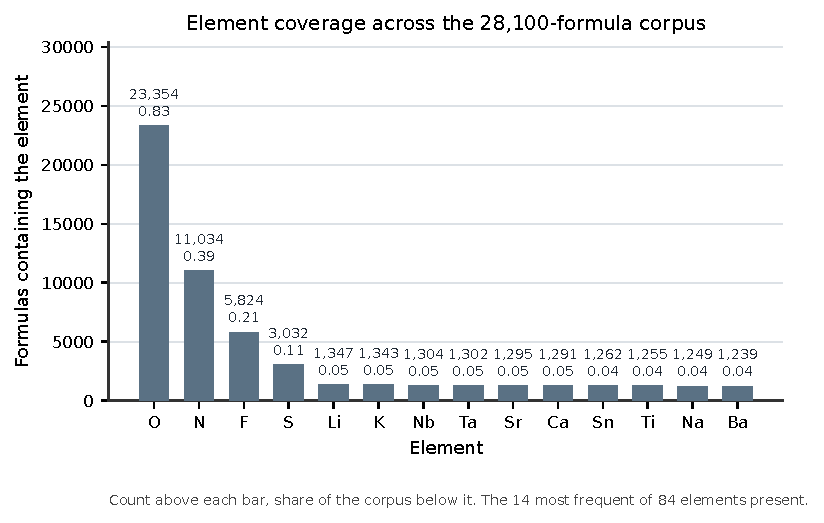
\includegraphics[width=0.8\textwidth]{paper2_element_coverage_origin_style.pdf}
\caption{Element coverage: distinct formulas containing each of the 14 most frequent of the 84 elements present.}\label{fig:s1}
\end{figure}
\begin{figure}[!h]\centering
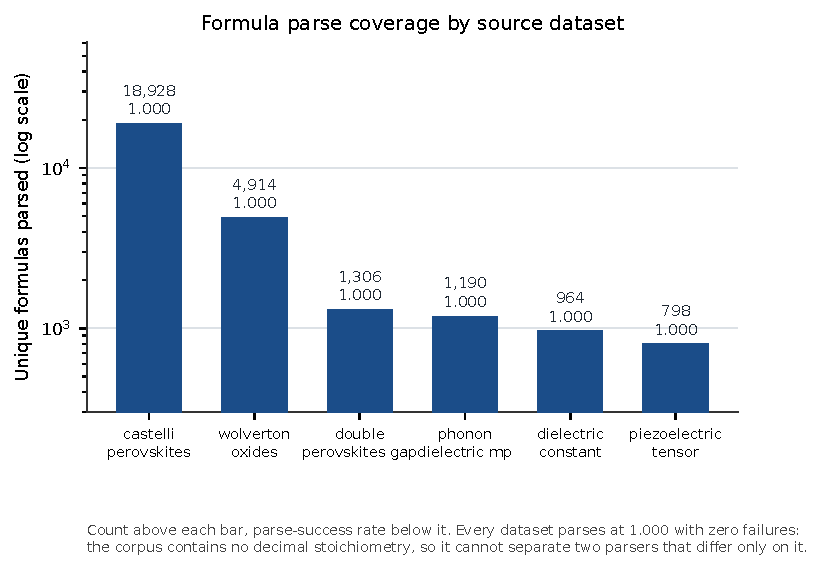
\includegraphics[width=0.8\textwidth]{paper2_parser_coverage_by_dataset_origin_style.pdf}
\caption{Unique formulas per dataset (log scale); every dataset parses completely under every configuration.}\label{fig:s2}
\end{figure}
\begin{figure}[!h]\centering
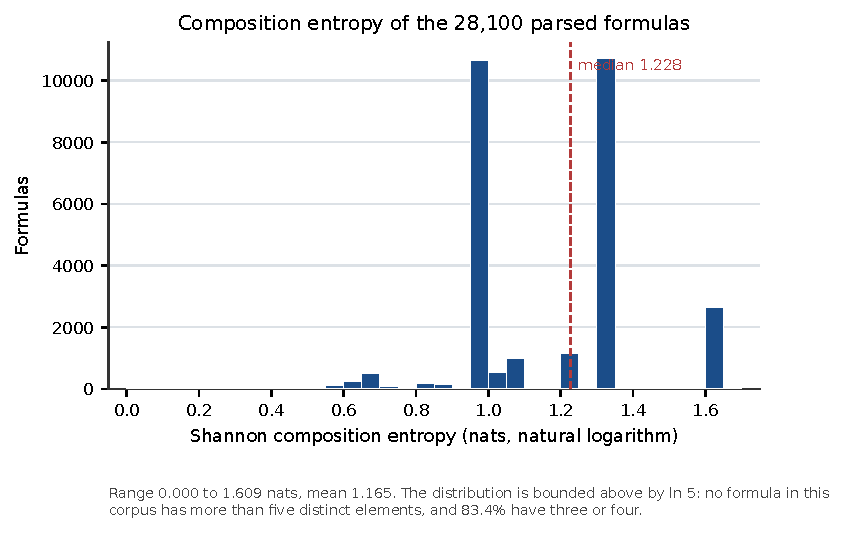
\includegraphics[width=0.8\textwidth]{paper2_formula_complexity_origin_style.pdf}
\caption{Distribution of composition entropy (nats) over the \NCorpus{} formulas; the dashed line marks the median, 1.228 nats.}\label{fig:s3}
\end{figure}

\section{Thesis-Derived Items}
\label{sec:s4}
The package descends from a thesis ratio parser. Six items were taken from the thesis text (Table~\ref{tab:s4}): three rule paragraphs that state a conversion but carry no formula instance, one fully normalized expression, one expression extracted with an ambiguity flag (the additive appears as \texttt{Y2} in the extracted text), and one workflow description. They are thesis-derived items, not six ratio expressions. Fig.~\ref{fig:s4} gives their status and Fig.~\ref{fig:s5} the atomic fractions of the one complete expression, as resolved by the v0.2.0 mixture layer.

\begin{table}[!h]\centering\footnotesize
\caption{The six thesis-derived items.}\label{tab:s4}
\begin{tabular}{@{}rlp{5.5cm}l@{}}
\toprule
Paragraph & Item type & Thesis expression & Status \\
\midrule
1411 & atomic\_percent\_rule & \texttt{chi at\% additive to host} & semantic\_rule\_extracted \\
1447 & molar\_percent\_rule & \texttt{chi mol\% additive to host} & semantic\_rule\_extracted \\
1498 & weight\_percent\_rule & \texttt{wt\% additive to host with molar-mass conversion} & semantic\_rule\_extracted \\
1519 & normalized\_mixture\_expression & \texttt{0.9977076(BaTiO3)+0.003924(Y2O3)+0.019(C)} & fully\_normalized\_expression\_parsed \\
1535 & atomic\_percent\_example & \texttt{(BaTiO3)+0.25at\%(Y2)} & semantic\_expression\_extracted\_with\_ambiguity \\
1548 & ratio\_parser\_workflow & \texttt{host/additive/alloying workflow for wt\%, at\%, and mol\%} & workflow\_rule\_extracted \\
\bottomrule
\end{tabular}

\end{table}
\begin{figure}[!h]\centering
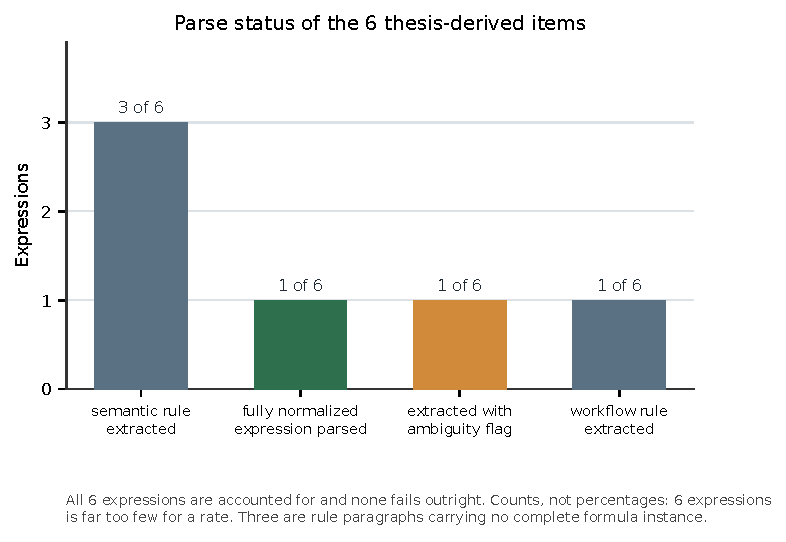
\includegraphics[width=0.7\textwidth]{paper2_thesis_ratio_status_origin_style.pdf}
\caption{Status of the six thesis-derived items, as counts.}\label{fig:s4}
\end{figure}
\begin{figure}[!h]\centering
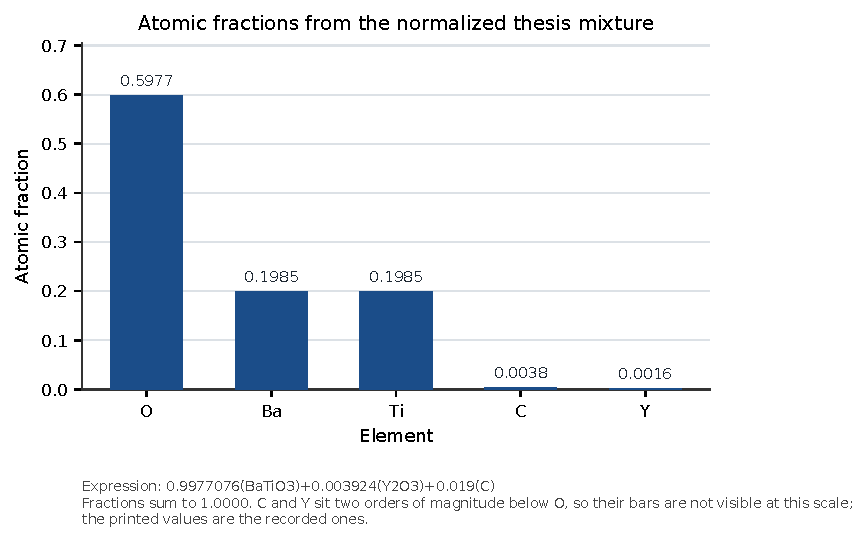
\includegraphics[width=0.7\textwidth]{paper2_thesis_mixture_atomic_fractions_origin_style.pdf}
\caption{Atomic fractions of \texttt{0.9977076(BaTiO3)+0.003924(Y2O3)+0.019(C)}: O 0.5977, Ba 0.1985, Ti 0.1985, C 0.0038, Y 0.0016 (symlog axis).}\label{fig:s5}
\end{figure}

\section{Downstream Illustration}
\label{sec:s5}
The submitted version reported a property-prediction check, which is retained here as an illustration only. It is not evidence for the parser, because every configuration compared in the main paper parses the \NDiel{} formulas of this dataset identically.

\paragraph{What was run.} The target was \texttt{poly\_total} from matminer's \texttt{dielectric\_constant} dataset~\cite{petousisS}, averaged per formula string, for the \NDiel{} formulas present in the parsed corpus. Two representations were compared: character 1--3-gram TF-IDF of the raw formula string, and the parsed atomic-fraction vector. The model was a random forest (scikit-learn, 100 trees, all other hyperparameters at their defaults, \texttt{random\_state}=42), scored by five-fold cross-validation with shuffled random folds (seed 42), in a single run. The cross-fold mean RMSE was 20.32 for TF-IDF and 19.10 for atomic fractions, and the MAE 7.84 and 6.33. No significance test was run.

\paragraph{Property availability.} The submitted Limitations section said that ``the underlying dielectric-constant property values'' were unavailable. That sentence referred only to a different, proposed comparison: features from \pmg alone against features from the fallback grammar alone, on formulas where the two backends disagree. No such formulas exist in the corpus, so that comparison is moot. The property values used for the check above were available when it was run.

\paragraph{Leakage across folds.} No two of the \NDiel{} records share a reduced composition (\NDielReduced{} distinct reduced compositions), so a random split cannot place the same composition in both training and test folds. They do, however, span only \NDielSystems{} chemical systems, and \NDielInSharedSystems{} records fall in \NDielSharedSystems{} systems that hold more than one record, such as Mn--O. A random split can therefore place closely related compositions on both sides.

\paragraph{Revised protocol.} The archive contains a script that repeats the check with folds grouped by chemical system (5 folds $\times$ 5 repeats). It compares TF-IDF, atomic fractions and matminer's Magpie \texttt{ElementProperty} statistics, using \texttt{RandomForestRegressor(n\_estimators=500, max\_features=1/3)}, and tests paired per-fold differences with the Wilcoxon signed-rank test. It verifies the property file against matminer's SHA-256 before running. Its results are not reported here, because the property file could not be retrieved in the environment used for the revision; they are not needed for any claim of the paper.

\section{Sample for Independent Expert Annotation}
\label{sec:s6}
The archive includes \NAnnotation{} literature strings drawn from both releases, stratified by notation stratum and reference class (up to 12 per cell, fixed seed). Each row gives the string and its DOI, with empty columns for two annotators, each recording a composition or a refusal decision, and an adjudication column. The protocol is for each annotator to read the string together with the cited article, independently, and record either the composition the authors meant or that the article does not determine one. Inter-annotator agreement would be reported as Cohen's $\kappa$ on the decision and as exact agreement on the compositions. These labels are not part of the present study.

\section{Reproduction}
\label{sec:s7}
\begin{enumerate}
\item Install the package with its pinned dependencies (\texttt{pymatgen} 2026.5.4, \texttt{pymatgen-core} 2026.8.30, matminer 0.10.1, pandas 2.2.3).
\item Fetch and verify the two literature releases from \url{https://github.com/CederGroupHub/text-mined-synthesis_public} at commit \texttt{fca0a994ddb36b37d39b803e8a21880aaecb1d71}.
\item Run the single entry point, which regenerates every result, table, figure and number macro of the paper, then run the test suite.
\end{enumerate}
The released parser and the version frozen for the first held-out run are each identified by SHA-256 in the archive. Every literature string's outcome under all five configurations is in the per-string CSV files, with controlled status and flags.

\begin{thebibliography}{1}
\bibitem{petousisS} I.~Petousis \emph{et al.}, ``High-throughput screening of inorganic compounds for the discovery of novel dielectric and optical materials,'' \emph{Scientific Data}, vol.~4, p.~160134, 2017, doi:10.1038/sdata.2016.134.
\end{thebibliography}
\end{document}
